\documentclass[a4paper,12pt]{article}
\usepackage[utf8]{inputenc}
\usepackage{hyperref}
\usepackage{graphicx,float}
\graphicspath{{images/}}
\usepackage[T1]{fontenc}
\usepackage[polish]{babel}
\usepackage{lmodern}
\usepackage[top=2cm,bottom=3cm,left=3cm,right=3cm]{geometry}
\usepackage{titlesec}
\usepackage{amsmath}
\usepackage{fancyvrb}
\usepackage{fvextra}
\titlelabel{\thetitle.\hspace{0.3em}}

\begin{document}
    \thispagestyle{empty}
    \vspace{1em}
    \noindent
    \begin{minipage}{0.48\textwidth}
        \raggedright
        Wydział: W4N\\Rok: 2025/2026\\Semestr: 5
    \end{minipage}
    \begin{minipage}{0.48\textwidth}
        \raggedleft
        Data oddania pracy:\\\today
    \end{minipage}
    \vspace{10em}
    \noindent
    \begin{center}
        \rule{\textwidth}{0.5pt}\\\vspace{2em}
        {\Huge\textbf{S}\Large\textbf{YSTEMY OPERACYJNE}}\\\vspace{1em}
        {\large\textbf{Część I: Dwukierunkowy dwuwątkowy algorytm Dijkstry}}\\\vspace{1em}
        {\large\textbf{Część II: Ucztujący filozofowie współbieżność}}\\\vspace{2em}
        \rule{\textwidth}{0.5pt}\\\vspace{4em}
        {\large Autor:}\\\vspace{0.5em}
        {\Large Kacper Piekut 280879}\\\vspace{3em}
        {\large Prowadzący:}\\\vspace{0.5em}
        {\Large dr Marek Bazan}
    \end{center}
    \vspace{3em}
    \begin{picture}(0,0)
        \put(0,-250){
\includegraphics[height=4cm]{logo pwr.png}}
    \end{picture}
    \newpage
    \section{Część I: Dwukierunkowy dwuwątkowy algorytm Dijkstry}
        \vspace{2em}
        \subsection{Wstęp}
            \vspace{1em}
            Algorytm Dijkstry jest jednym z najważniejszych i najczęściej stosowanych algorytmów grafowych służących do wyznaczania najkrótszych ścieżek w grafach o nieujemnych wagach krawędzi. Znajduje szerokie zastosowanie w informatyce, m.in. w systemach nawigacyjnych, sieciach komputerowych czy optymalizacji tras. Klasyczna wersja algorytmu działa w sposób jednowątkowy, co może prowadzić do ograniczeń wydajnościowych przy przetwarzaniu dużych grafów. W odpowiedzi na te wyzwania powstały różne podejścia do równoległego przetwarzania, w tym dwukierunkowy algorytm Dijkstry, który wykorzystuje dwa wątki do jednoczesnego poszukiwania najkrótszej ścieżki od źródła do celu oraz od celu do źródła. Takie podejście może znacząco przyspieszyć proces znajdowania najkrótszej ścieżki, zwłaszcza w dużych i złożonych grafach.
            \vspace{2em}
        \subsection{Cele projektu}
            \vspace{1em}
            Celem projektu jest zaimplementowanie i przetestowanie algorytmu Dijkstry w wersji jednowątkowej oraz dwuwątkowej w języku C++. Projekt zakłada:
            \begin{itemize}
                \item stworzenie generatora losowych grafów skierowanych o zadanych parametrach,
                \item implementację klasycznego algorytmu Dijkstry oraz jego wersji dwuwątkowej,
                \item pomiar i porównanie czasów działania obu wersji algorytmu dla różnych rozmiarów grafów i gęstości krawędzi,
                \item analizę poprawności wyznaczanych ścieżek i wyników,
                \item ocenę korzyści z zastosowania wielowątkowości w praktyce.
            \end{itemize}
        \newpage
        \vspace*{2em}
        \subsection{Plan eksperymentu}
            \vspace{1em}
        	\textbf{Testowany algorytm}\\
            \vspace{-1.0em}\\
            Testowany jest klasyczny algorytm Dijkstry w wersji jednowątkowej oraz jego wariant dwuwątkowy. Obie wersje korzystają z kolejki priorytetowej i operują na grafie skierowanym o nieujemnych wagach krawędzi. Algorytmy wyznaczają najkrótszą ścieżkę pomiędzy wybranymi wierzchołkami grafu.\\
            \vspace{0.5em}\\
        	\textbf{Dane wejściowe i generowanie grafów}\\
            \vspace{-1.0em}\\
            Dane wejściowe stanowią losowo generowane grafy skierowane o zadanej liczbie wierzchołków i gęstości krawędzi w postaci macierzowej reprezentacji. Grafy są generowane automatycznie przez program. Wagi krawędzi są losowane z ustalonego zakresu liczb całkowitych.\\
            \vspace{0.5em}\\
        	\textbf{Środowisko testowe}\\
            \vspace{-0.5em}\\
            Eksperyment jest wykonywany w środowisku konsolowym na komputerze z systemem Windows. Kod został napisany w języku C++ i kompilowany przy użyciu kompilatora MinGW (GCC) w wersji 13.2.0. Wyniki mogą być zależne od wydajności sprzętu, dlatego wnioski dotyczące efektywności algorytmów są formułowane w sposób ogólny.\\
            \vspace{1em}\\
        	\textbf{Specyfikacja sprzętowa}\\
            \vspace{-0.5em}\\
            Laptop: ASUS TUF Gaming F15.\\
            Procesor: Intel Core i5-11400H, 6 rdzeni, 12 wątków, taktowanie bazowe 2.7 GHz (do 4.5 GHz w trybie turbo).\\
            Pamięć RAM: 16 GB DDR4.\\
            Dysk: SSD NVMe 512 GB (Samsung MZVLQ512HBLU-00B00).\\
            Karta graficzna: NVIDIA GeForce RTX 3050 Laptop GPU\\oraz Intel UHD Graphics.\\
            System operacyjny: Microsoft Windows 11 Home 64-bit, wersja 10.0.26100.
        \newpage
        \vspace*{2em}
        \subsection{Implementacja}
            \vspace{1em}
            Program testuje algorytm Dijkstry w wersji jednowątkowej i dwuwątkowej, korzystając z biblioteki STL oraz mechanizmów wielowątkowości C++.\\\\
            \textbf{Zmienne globalne:}
                \begin{itemize}
                    \item \textbf{INF} - stała oznaczająca nieskończoność (brak ścieżki),
                    \item \textbf{path\_single, path\_double} - wektory przechowujące wyznaczone ścieżki dla wersji jednowątkowej i dwuwątkowej.
                \end{itemize}
            \textbf{Funkcja generateGraph} - generuje skierowany graf o liczbie wierzchołków n i gęstości d w macierzowej reprezentacji (vector<vector<int>>), gdzie INF oznacza brak krawędzi, a na przekątnej znajdują się zera. Funkcja wspiera tryb siatki (grid):
                \begin{itemize}
                    \item w trybie grid budowana jest siatka 2D z krawędziami tylko w prawo i w dół (skierowane), wagi losowane z przedziału $[1, n]$;
                    \item następnie dobija się wymaganą gęstość losowymi krawędziami o wagach z przedziału $[1, 2n]$ (większy zakres dla krawędzi dodatkowych);
                    \item w trybie losowym (bez gridu) generowane są krawędzie z wagami $[1, n]$.
                \end{itemize}
                \textbf{Funkcja pomocnicza reconstruct\_path} - rekonstruuje ścieżkę z tablic rodziców wyznaczonych przez przeszukiwania od początku i od końca.\\
                \vspace{-0.5em}\\
                \textbf{Funkcja dijkstraSingle} - jednowątkowa wersja z dwukierunkowym przeszukiwaniem. Budowana jest odwrócona macierz, utrzymywane są dwie kolejki priorytetowe (front od początku i od końca), a warunek szybkiego zakończenia porównuje najmniejsze klucze w kolejkach z aktualnym best (najlepszym znalezionym dystansem). Po wyznaczeniu punktu spotkania meet ścieżka jest rekonstruowana.\\
                \vspace{-0.5em}\\
                \textbf{Funkcja dijkstraDouble} - wersja dwuwątkowa. Dwa wątki niezależnie przeszukują graf (macierz i jej odwrócenie), współdzieląc best, meet i flagę stop. Synchronizacja tych zmiennych odbywa się za pomocą mutex; wątek może zakończyć pracę wcześniej, gdy dalsze ulepszanie best nie jest możliwe.\\
                \vspace{-0.5em}\\
                \textbf{Funkcja measureTime} - mierzy czas wykonania przekazanej funkcji i zwraca wynik w milisekundach (high\_resolution\_clock).\\
                \vspace{-0.5em}\\
                \textbf{Funkcja main} - inicjalizacja, pętle testowe dla zestawów $n$ i $d$, włączenie trybu siatki (grid), ustawienie start=0, end=n-1 w trybie grid, uruchomienie obu wersji algorytmu, weryfikacja poprawności (porównanie dystansów), agregacja i wypis wyników (w tym proporcji czasu jednowątkowego do dwuwątkowego).\\
            \newpage
            \vspace*{2em}
            \hspace{-1.5em}\textbf{Struktura danych:}
            \begin{itemize}
                \item Graf: vector<vector<int>> - macierz sąsiedztwa z wagami; INF oznacza brak krawędzi. Dla przeszukiwania od końca budowana jest odwrócona macierz.
                \item Kolejki priorytetowe: priority\_queue<pair<int,int>, vector<pair<int,int>>, greater<pair<int,int>> - wybór wierzchołka o najmniejszej odległości w obu kierunkach.
                \item Tablice odległości i rodziców: vector<int> - przechowują aktualne odległości od początku/końca oraz poprzedników na ścieżce.
            \end{itemize}
            \vspace{1em}
            \textbf{Wielowątkowość:}
            \begin{itemize}
                \item Wersja dwuwątkowa używa std::thread do równoległego uruchomienia dwóch przeszukiwań; kluczowe zmienne współdzielone są chronione przez mutex.
                \item Po zakończeniu pracy wątków wykonywany jest join(), a następnie następuje rekonstrukcja ścieżki.
            \end{itemize}
            \vspace{1em}
            \textbf{Obsługa pomiarów i prezentacja wyników:}
            \begin{itemize}
                \item Dla każdej konfiguracji (rozmiar grafu, gęstość) wykonywanych jest 10 prób, a wyniki są uśredniane.
                \item Program wypisuje na konsolę średnie czasy działania obu wersji algorytmu dla każdej konfiguracji.
                \item Opcjonalnie możliwe jest wypisanie wygenerowanego grafu oraz wyznaczonych ścieżek.
            \end{itemize}
            \vspace{1em}
        \newpage
        \vspace*{2em}
        \subsection{Badania}
            \vspace{1em}
            W celu porównania wydajności klasycznego (jednowątkowego) oraz dwuwątkowego algorytmu Dijkstry przeprowadzono serię testów na losowo generowanych grafach skierowanych o różnych rozmiarach ($n$) i gęstościach ($d$). Dla każdej konfiguracji przeprowadzono po 10 testów, których został wyciągnięty średni czas wykonania się algorytmu obu wersji. Wyniki przedstawiono w poniższej tabeli.
            \begin{table}[H]
                \centering
                \hspace*{-1em}\begin{tabular}{|c|c|c|c|c|}
                    \hline
                    Liczba wierzchołków $n$ & Gęstość $d$ & Średni czas I [ms] & Średni czas II [ms] & Różnica \\
                    \hline
                    500   & 0.01 & 3.1   & 2.3   & 1.34 \\
                    500   & 0.25 & 6.0   & 4.3   & 1.39 \\
                    500   & 0.50 & 8.3   & 6.6   & 1.25 \\
                    500   & 0.75 & 7.0   & 5.1   & 1.37 \\
                    500   & 0.90 & 6.0   & 4.5   & 1.33 \\
                    1000  & 0.01 & 11.5  & 6.5   & 1.76 \\
                    1000  & 0.25 & 20.2  & 11.4  & 1.77 \\
                    1000  & 0.50 & 27.4  & 16.0  & 1.71 \\
                    1000  & 0.75 & 24.9  & 14.5  & 1.71 \\
                    1000  & 0.90 & 21.6  & 13.2  & 1.63 \\
                    5000  & 0.01 & 270.2  & 164.8 & 1.63 \\
                    5000  & 0.25 & 488.6  & 296.1  & 1.65 \\
                    5000  & 0.50 & 700.8  & 425.2  & 1.64 \\
                    5000  & 0.75 & 615.3  & 388.1  & 1.58 \\
                    5000  & 0.90 & 543.3  & 376.4  & 1.44 \\
                    10000 & 0.01 & 1169.8 & 862.2  & 1.35 \\
                    10000 & 0.25 & 2274.5 & 1677.8 & 1.35 \\
                    10000 & 0.50 & 3210.2 & 2282.2 & 1.4 \\
                    10000 & 0.75 & 2913.7 & 2152.0 & 1.35 \\
                    10000 & 0.90 & 2706.1 & 2103.4 & 1.28 \\
                    20000 & 0.01 & 4903.8 & 3633.9 & 1.34 \\
                    20000 & 0.25 & 10352.1 & 7770.0 & 1.32 \\
                    20000 & 0.50 & 13335.8 & 10318.9 & 1.29 \\
                    20000 & 0.75 & 14053.5 & 10724.6 & 1.31 \\
                    20000 & 0.90 & 13080.4 & 10560 & 1.23 \\
                    \hline
                \end{tabular}
                \caption{Porównanie średnich czasów wykonania algorytmu Dijkstry w wersji jednowątkowej (I) i dwuwątkowej (II) dla różnych rozmiarów i gęstości grafu oraz stosunek I/II (Różnica).}
            \end{table}

            \begin{figure}[H]
                \centering
                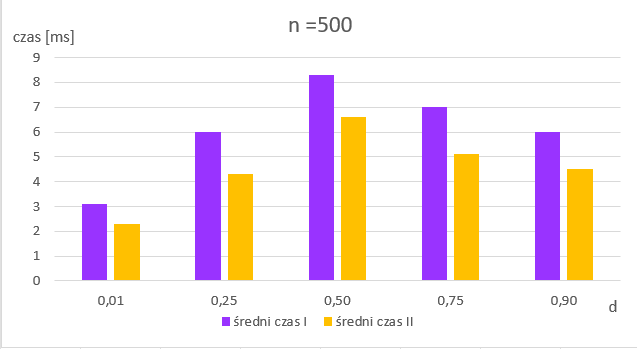
\includegraphics[width=0.7\textwidth]{wykres_n=500.png}
                \caption{Porównanie czasów dla $n=500$}
            \end{figure}
            \begin{figure}[H]
                \centering
                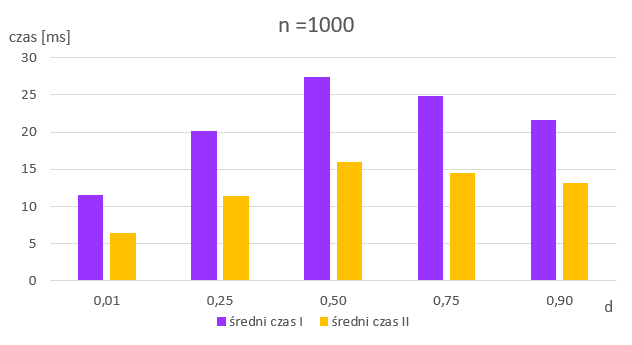
\includegraphics[width=0.7\textwidth]{wykres_n=1000.png}
                \caption{Porównanie czasów dla $n=1000$}
            \end{figure}
            \begin{figure}[H]
                \centering
                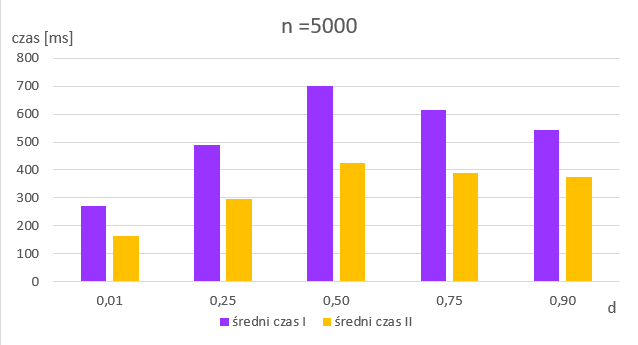
\includegraphics[width=0.7\textwidth]{wykres_n=5000.png}
                \caption{Porównanie czasów dla $n=5000$}
            \end{figure}
            \begin{figure}[H]
                \centering
                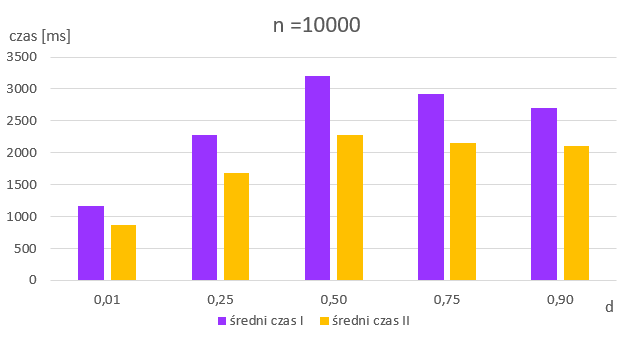
\includegraphics[width=0.7\textwidth]{wykres_n=10000.png}
                \caption{Porównanie czasów dla $n=10000$}
            \end{figure}
            \begin{figure}[H]
                \centering
                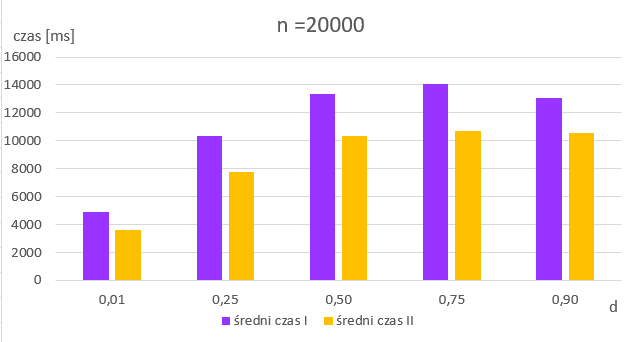
\includegraphics[width=0.7\textwidth]{wykres_n=20000.png}
                \caption{Porównanie czasów dla $n=20000$}
            \end{figure}
        \newpage
        \vspace*{2em}
        \subsection{Wnioski}
            \vspace{1em}
            Wyniki aktualnych pomiarów pokazują, że dwukierunkowa wersja algorytmu jest konsekwentnie szybsza od jednowątkowej we wszystkich badanych konfiguracjach. Zarejestrowane proporcje czasu I/II mieszczą się najczęściej w przedziale 1.3-1.7, a maksymalny odnotowany zysk wyniósł \textbf{1.77} (dla $n=1000$, $d=0{,}25$).
            \begin{itemize}
                \item \textbf{Wpływ gęstości:} największe przyspieszenia uzyskiwano dla umiarkowanej gęstości (np. $d=0{,}25$). Dla bardzo rzadkich ($d=0{,}01$) oraz bardzo gęstych ($d=0{,}9$) grafów zysk był mniejszy (zwykle 1.2-1.35). Wynika to z krótszych tras i szybszego domknięcia best, co ogranicza zakres równoległego przeszukiwania.
                \item \textbf{Wpływ rozmiaru:} wraz ze wzrostem $n$ czasy rosną, ale stosunek I/II pozostaje stabilny i najczęściej mieści się w zakresie 1.3-1.6. Przy największym rozmiarze ($n=20000$) dla $d=0{,}25$ zanotowano zysk na poziomie 1.33, a dla $d=0{,}75$ 1.31.
                \item \textbf{Jednowątkowy vs. narzuty:} przy małych $n$ różnice są ograniczone przez narzuty uruchomienia wątków i synchronizacji, jednak nadal obserwuje się przewagę wersji dwuwątkowej.
                \item \textbf{Struktura grafu:} tryb grid (krawędzie prawo/dół, wagi $[1,n]$) wymusza trasy z większą liczbą wyrzchołków na trasie, co sprzyja dwukierunkowości. Dodatkowe krawędzie o większym zakresie wag rzadziej tworzą opłacalne skróty.
            \end{itemize}
        \newpage
        \vspace*{2em}
        \subsection{Podsumowanie}
            \vspace{1em}
            Zaimplementowano dwie wersje algorytmu Dijkstry (jednowątkową i dwuwątkową - dwukierunkowe) działające na macierzowej reprezentacji grafu. Obie wersje zwracają zgodne długości najkrótszych ścieżek, a pomiary potwierdzają systematyczny zysk czasowy wariantu dwuwątkowego - najczęściej 1.3-1.7, lokalnie do \textbf{1.77}. Skuteczność rośnie dla umiarkowanych gęstości i większych rozmiarów, maleje dla skrajnych gęstości.\\
            \vspace{0.5em}\\
            Ograniczenia w osiąganiu pełnego dwukrotnego przyśpieszenia wynikają m.in. z narzutów synchronizacji, kosztów operacji na priority\_queue oraz skanowania wierszy macierzy (koszt per wierzchołek niezależny od stopnia).
            \vspace{1.5em}
        \subsection{Literatura}
            \vspace{1em}
            \begin{itemize}
                \item \url{https://pl.wikipedia.org/wiki/Algorytm_Dijkstry}
                \item \url{https://en.wikipedia.org/wiki/Dijkstra%27s_algorithm}
                \item Mirosław Zelent kurs C++ \url{https://miroslawzelent.pl/kurs-c++/}
            \end{itemize}
        \newpage
        \vspace*{2em}
        \subsection{Kod}
            \vspace{1em}
            \VerbatimInput[frame=single,numbers=left,breaklines=true,breakanywhere=true,tabsize=4]{../dikstra.cpp}
    \newpage
    \section{Część II: Ucztujący filozofowie współbieżność}
        \vspace{2em}
        \subsection{Wstęp}
            \vspace{1em}
            Problem ucztujących filozofów jest jednym z klasycznych zagadnień synchronizacji w programowaniu współbieżnym. Został sformułowany przez Edsgera Dijkstrę jako ilustracja problemów związanych z dostępem do współdzielonych zasobów przez wiele procesów. Ucztujący filozofowie są metaforą dla procesów konkurujących o ograniczone zasoby, takie jak np. drukarki, pliki czy inne urządzenia peryferyjne. Niewłaściwa synchronizacja może prowadzić do sytuacji, w której żaden z procesów nie może kontynuować pracy (zakleszczenie) lub niektóre procesy są stale pomijane (zagłodzenie). Analiza i implementacja tego problemu pozwala lepiej zrozumieć mechanizmy synchronizacji, takie jak semafory czy muteksy czy, oraz uczy projektowania algorytmów odpornych na typowe błędy współbieżności.
            Wersja zadania zakłada, że N filozofów siedzi przy okrągłym stole, a pomiędzy każdym z nich leży jeden widelec. Każdy filozof naprzemiennie myśli i je, a do jedzenia potrzebuje dwóch widelców - lewego i prawego.
        \vspace{2em}
        \subsection{Cele projektu}
            \vspace{1em}
            Celem projektu jest zaimplementowanie wielowątkowej symulacji problemu ucztujących filozofów w języku C++. Program ma umożliwiać obserwację zachowania filozofów oraz poprawnie synchronizować dostęp do współdzielonych zasobów (widelców), tak aby:
            \begin{itemize}
                \item zapobiec zakleszczeniu,
                \item zminimalizować ryzyko zagłodzenia,
                \item umożliwić równoległe działanie wielu wątków,
                \item zilustrować praktyczne aspekty synchronizacji w programowaniu współbieżnym.
            \end{itemize}
        \newpage
        \vspace*{2em}
        \subsection{Plan eksperymentu}
            \vspace{1em}
        	\textbf{Testowany kod i scenariusz}\\
            \vspace{-1.0em}\\
            Testowany jest program symulujący problem ucztujących filozofów, w którym każdy filozof jest reprezentowany przez osobny wątek. Synchronizacja dostępu do widelców realizowana jest za pomocą mutexów oraz własnej implementacji semafora licznikowego. Program umożliwia wykrywanie zagłodzenia.\\
            \vspace{0.5em}\\
        	\textbf{Dane wejściowe i parametry}\\
            \vspace{-1.0em}\\
            Dane wejściowe stanowią liczba filozofów (domyślnie 100), czas trwania symulacji oraz parametry dotyczące czasu myślenia i jedzenia (losowane z ustalonych zakresów). Program umożliwia modyfikację tych parametrów w celu obserwacji różnych scenariuszy synchronizacji i ryzyka zagłodzenia.\\
            \vspace{0.5em}\\
        	\textbf{Środowisko testowe}\\
            \vspace{-0.5em}\\
            Eksperyment jest wykonywany w środowisku konsolowym na komputerze z systemem Windows. Kod został napisany w języku C++ i kompilowany przy użyciu kompilatora MinGW (GCC) w wersji 13.2.0. Wyniki mogą być zależne od wydajności sprzętu, dlatego wnioski dotyczące efektywności algorytmów są formułowane w sposób ogólny.\\
            \vspace{1em}\\
        	\textbf{Specyfikacja sprzętowa}\\
            \vspace{-0.5em}\\
            Laptop: ASUS TUF Gaming F15.\\
            Procesor: Intel Core i5-11400H, 6 rdzeni, 12 wątków, taktowanie bazowe 2.7 GHz (do 4.5 GHz w trybie turbo).\\
            Pamięć RAM: 16 GB DDR4.\\
            Dysk: SSD NVMe 512 GB (Samsung MZVLQ512HBLU-00B00).\\
            Karta graficzna: NVIDIA GeForce RTX 3050 Laptop GPU\\oraz Intel UHD Graphics.\\
            System operacyjny: Microsoft Windows 11 Home 64-bit, wersja 10.0.26100.
        \newpage
        \vspace*{2em}
        \subsection{Implementacja}
            \vspace{1em}
            Implementacja problemu ucztujących filozofów została zrealizowana w języku C++ z wykorzystaniem wątków oraz mechanizmów synchronizacji dostępnych w standardowej bibliotece. Każdy filozof jest reprezentowany przez osobny wątek, który cyklicznie przechodzi przez stany: myślenie, głód oraz jedzenie.\\
            \vspace*{1em}\\
        	\hspace{-0.5em}\textbf{Główne zmienne i struktury:}
            \begin{itemize}
                \item int threads - liczba filozofów oraz widelców (domyślnie 100).
                \item vector<thread> thread\_vec - wektor przechowujący obiekty wątków, po jednym dla każdego filozofa.
                \item vector<mutex> sticks - wektor mutexów reprezentujących widelce leżące pomiędzy filozofami.
                \item atomic\_bool thread\_check - flaga sterująca zakończeniem działania wszystkich wątków.
                \item mutex print\_mutex - mutex do synchronizacji wypisywania komunikatów na konsolę.
                \item Semaphore sem - własna implementacja semafora licznikowego ograniczającego liczbę filozofów próbujących jeść (zalecane: Semaphore sem(threads-1)).
            \end{itemize}
            \vspace{1.5em}
        	\textbf{Kluczowe funkcje:}
            \begin{itemize}
                \item void philosopherLoop(const int id) - funkcja wykonywana przez każdy wątek-filozofa. Zawiera główną pętlę: myślenie (losowy czas), wypisanie stanu głodu, próba zdobycia widelców (mutexy), jedzenie (czas jak myślenia), wypuszczenie widelców, powrót do myślenia. Zawiera także mechanizm wykrywania zagłodzenia (jeśli filozof czeka ponad 10 sekund na możliwość jedzenia, program zostaje przerwany).
                \item int main() - inicjalizuje zmienne globalne, uruchamia wątki filozofów, czeka określony czas trwania symulacji, a następnie kończy wszystkie wątki i dołącza je do głównego programu.
            \end{itemize}
        	\newpage
        	\vspace*{4em}
            \hspace{-1.5em}\textbf{Synchronizacja, unikanie zakleszczenia i zagłodzenia:}
            \begin{itemize}
                \item Każdy filozof przed próbą podniesienia widelców wywołuje sem.try\_acquire() w pętli, co pozwala wykryć zagłodzenie (limit czasu oczekiwania).
                \item Widelce są blokowane przez wywołanie std::lock(sticks[left],\\sticks[right]), co zapobiega zakleszczeniu na poziomie mutexów.
                \item Po zakończeniu jedzenia mutexy są odblokowywane, a semafor zwalniany przez sem.release().
                \item Wszystkie wypisy na konsolę są chronione przez print\_mutex, aby uniknąć mieszania się komunikatów z różnych wątków.
            \end{itemize}
            \vspace{1.5em}
        	\textbf{Opis działania semafora:}
            \begin{itemize}
                \item Klasa Semaphore wykorzystuje mutex i condition\_variable do implementacji licznika dostępnych "pozwoleń".
                \item Metoda acquire() blokuje wątek, jeśli nie ma dostępnych pozwoleń, a\\release() je zwalnia i powiadamia czekające wątki.
                \item Metoda try\_acquire() pozwala nieblokująco sprawdzić dostępność semafora (używana do wykrywania zagłodzenia).
            \end{itemize}
            \vspace{1.5em}
        	\textbf{Losowanie czasu:}
            \begin{itemize}
                \item Czas myślenia każdego filozofa jest losowany z przedziału 1-5 sekund przy użyciu funkcji rand().
                \item Czas jedzenia jest równy czasowi myślenia z danej iteracji.
            \end{itemize}
        \newpage
        \vspace*{2em}
        \subsection{Badania}
            \vspace{1em}
            W ramach badań przeprowadzono serię eksperymentów z różną liczbą filozofów (5, 10, 50, 100) oraz różnymi ustawieniami semafora ograniczającego liczbę filozofów próbujących jeść jednocześnie. Celem było zaobserwowanie, jak zmiana tych parametrów wpływa na występowanie zakleszczenia i zagłodzenia oraz na ogólne zachowanie programu. Czas każdej symulacji ustawiono na 60 sekund.
        	\vspace{1.5em}
            \begin{table}[H]
                \centering
                \begin{tabular}{|c|c|c|c|}
                    \hline
                    Liczba filozofów ($n$) & Ograniczenie semafora & Zagłodzenie & Zakleszczenie \\
                    \hline
                    10 & [$\frac{1}{3} \cdot n$] & wystąpiło & brak \\
                    10 & [$\frac{1}{2} \cdot n$] & wystąpiło & brak \\
                    10 & n - 1 & brak & brak \\
                    50 & [$\frac{1}{3} \cdot n$] & wystąpiło & brak \\
                    50 & [$\frac{1}{2} \cdot n$] & wystąpiło & brak \\
                    50 & n - 1 & brak & brak \\
                    100 & [$\frac{1}{3} \cdot n$] & wystąpiło & brak \\
                    100 & [$\frac{1}{2} \cdot n$] & wystąpiło & brak \\
                    100 & n - 1 & brak & brak \\
                    \hline
                \end{tabular}
                \caption{Wyniki eksperymentów dla różnych parametrów symulacji}
            \end{table}
        \newpage
        \vspace*{2em}
        \subsection{Wnioski}
            \vspace{1em}
            Przeprowadzone eksperymenty potwierdziły, że odpowiednie ustawienie ograniczenia semafora ma kluczowe znaczenie dla poprawnego działania algorytmu ucztujących filozofów. Zbyt mała wartość semafora prowadzi do zagłodzenia niektórych wątków, natomiast ustawienie go na $n-1$ (gdzie $n$ to liczba filozofów) skutecznie eliminuje zagłodzenie. Mechanizm wykrywania zagłodzenia pozwala łatwo zidentyfikować niepoprawne ustawienia synchronizacji i potwierdzić poprawność działania programu. Zakleszczenie nie wystąpiło w żadnym z testów dzięki zastosowaniu semafora oraz odpowiedniej kolejności blokowania mutexów.
            \vspace{1.5em}
        \subsection{Podsumowanie}
            \vspace{1em}
            Problem ucztujących filozofów jest klasycznym przykładem wyzwań związanych z synchronizacją w programowaniu współbieżnym. Przeprowadzona implementacja i badania pokazały, że stosując prosty semafor licznikowy oraz odpowiednie techniki synchronizacji, można skutecznie zapobiec zakleszczeniu i zagłodzeniu. Eksperymenty wykazały, że poprawne ustawienie parametrów synchronizacji jest kluczowe dla zapewnienia sprawiedliwego dostępu do zasobów przez wszystkie wątki. Opracowany program pozwala na łatwą obserwację i analizę działania algorytmów synchronizacyjnych w praktyce.
            \vspace{1.5em}
        \subsection{Literatura}
            \vspace{1em}
            \begin{itemize}
                \item \url{https://pl.wikipedia.org/wiki/Problem_ucztujących_filozofów}
                \item \url{https://en.wikipedia.org/wiki/Dining_philosophers_problem}
                \item Mirosław Zelent kurs C++ \url{https://miroslawzelent.pl/kurs-c++/}
            \end{itemize}
        \newpage
        \vspace*{2em}
        \subsection{Kod}
            \vspace{1em}
            \VerbatimInput[frame=single,numbers=left,breaklines=true,breakanywhere=true,tabsize=4]{../filozofowie.cpp}
\end{document}
